%##################################################################################################
\begin{table*}[t]
\centering
\subfloat[
    \textbf{CIFAR-10 (5+5).} ResNet-20 (4$\times$ width).
    \label{tab:cifar5+5}
]{
\centering
\begin{minipage}{0.47\linewidth}{
\begin{center}
\resizebox{\textwidth}{!}{
    \tablestyle{5pt}{1.1}
    \begin{tabular}{lc|cccc}
        & & \multicolumn{4}{c}{Accuracies (\%)}\\
        Method & FLOPs (G) & Joint & \modela{Task A} & \modelb{Task B} & Avg \\
        \shline
        \modela{Model A} & {0.68} & {48.2\conf{1.0}} & {97.0\conf{0.6}} & {45.1\conf{8.6}} & {71.0\conf{4.4}} \\
        \modelb{Model B} & {0.68} & {48.4\conf{3.8}} & {49.1\conf{9.3}} & {96.1\conf{1.1}} & {72.6\conf{4.9}} \\
        \hline
        W. Avg \tiny{(Eq.~\ref{eq:wavg})} & 0.68 & {43.0\conf{1.6}} & {54.1\conf{1.4}} & {67.5\conf{1.2}} & {60.8\conf{4.5}} \\
        % Git Re-Basin \cite{ainsworth2022git}  & 0.68 & {46.2\conf{0.8}} & {76.8\conf{8.9}} & {82.7\conf{5.1}} & {79.8\conf{6.5}} \\
        Git Re-Basin$^{\ddag}$  & 0.68 & {46.2\conf{0.8}} & {76.8\conf{8.9}} & {82.7\conf{5.1}} & {79.8\conf{6.5}} \\
        Permute \tiny{(Eq.~\ref{eq:rebasin})} & 0.68 & {58.4\conf{6.8}} & {86.6\conf{2.1}} & {87.4\conf{1.1}} & {87.4\conf{1.4}} \\
        \default{{\bf \name{}}$_\text{20/20}$} & 0.68 & \textbf{79.1\conf{1.1}} & \textbf{92.9\conf{1.1}} & \textbf{91.2\conf{1.4}} & \textbf{92.1\conf{1.0}} \\
        \hline
        \gc{Ensemble} & \gc{1.37} & \gc{87.4\conf{2.6}} & \gc{97.0\conf{0.6}} & \gc{96.1\conf{1.1}} & \gc{96.6\conf{0.4}} \\
        \default{{\bf \name{}}$_\text{13/20}$} & 0.91 & \textbf{83.8\conf{3.1}} & \textbf{95.1\conf{0.7}} & \textbf{94.1\conf{1.5}} & \textbf{94.6\conf{0.6}} \\
    \end{tabular}
}
\end{center}
}\end{minipage}
}
\hspace{1em}
\centering
\subfloat[
    \textbf{CIFAR-100 (50+50).} ResNet-20 (8$\times$ width).
    \label{tab:cifar50+50}
]{
\centering
\begin{minipage}{0.47\linewidth}{
\begin{center}
\resizebox{\textwidth}{!}{
    \tablestyle{5pt}{1.1}
    \begin{tabular}{y{53}x{40}|x{30}x{30}x{30}x{30}}
        & & \multicolumn{4}{c}{Accuracies (\%)}\\
        Method & FLOPs (G) & Joint & \modela{Task A} & \modelb{Task B} & Avg \\
        \shline
        \modela{Model A} & {2.72} & {41.6\conf{0.3}} & {82.9\conf{0.7}} & {24.8\conf{0.4}} & {53.9\conf{0.5}} \\
        \modelb{Model B} & {2.72} & {41.6\conf{0.2}} & {25.1\conf{1.2}} & {82.8\conf{0.2}} & {54.0\conf{0.6}} \\
        \hline
        W. Avg \tiny{(Eq.~\ref{eq:wavg})}             &  2.72     & {17.0\conf{1.7}}          & {23.8\conf{6.9}}     & {24.8\conf{5.9}} & {24.3\conf{1.9}} \\
        % Git Re-Basin \cite{ainsworth2022git}        &  2.72     & {40.9\conf{0.2}}          & {57.3\conf{1.5}}      & {56.7\conf{0.7}}  & {57.0\conf{0.8}}  \\
        Git Re-Basin$^{\ddag}$    &  2.72     & {40.9\conf{0.2}}          & {57.3\conf{1.5}}      & {56.7\conf{0.7}}  & {57.0\conf{0.8}}  \\
        Permute \tiny{(Eq.~\ref{eq:rebasin})}    &  2.72     & {42.8\conf{0.7}}          & {61.6\conf{1.4}}      & {60.5\conf{0.5}}   & {61.0\conf{0.8}} \\
        \default{{\bf \name{}}$_\text{20/20}$}  &  2.72   & \textbf{54.9\conf{0.8}}          & \textbf{68.2\conf{0.8}}      & \textbf{67.9\conf{0.6}}  & \textbf{68.0\conf{0.4}} \\
        \hline
        \gc{Ensemble}                           & \gc{5.45} & \gc{73.5\conf{0.4}}       & \gc{82.9\conf{0.7}}   & \gc{82.8\conf{0.2}}& \gc{82.8\conf{0.4}} \\
        \default{{\bf \name{}}$_\text{13/20}$}  & {3.63}    & \textbf{70.2\conf{0.4}}   & \textbf{80.3\conf{0.8}}      & \textbf{80.1\conf{0.7}}  & \textbf{80.2\conf{0.6}} \\
    \end{tabular}
}
\end{center}
}\end{minipage}
}
\caption{\textbf{CIFAR Results.} \name{}\ vs.\ baselines
on combining a model trained on half the classes (\modela{Task A}) with one trained on the other half (\modelb{Task B}) \textit{without extra training}. We report both joint (10/100-way) and per-task (5/50-way) accuracy.
\name{}\ \textit{significantly} outperforms its baseline and closes in on the \gc{upper bound} (ensemble accuracy).
$\ddag$ refers to \citet{ainsworth2022git}.
}
\label{tab:cifar_results}
\vspace{-15pt}
\end{table*}
%##################################################################################################


% %##################################################################################################
% \begin{table*}[t]
% \centering
% \subfloat[
%     \textbf{CIFAR-10 (5+5).} Using ResNet-20 (4$\times$ width).
%     \label{tab:cifar5+5}
% ]{
% \centering
% \begin{minipage}{0.46\linewidth}{
% \begin{center}
% \resizebox{\textwidth}{!}{
%     \tablestyle{5pt}{1.1}
%     \begin{tabular}{y{56}x{20}x{28}|x{24}x{24}x{24}}
%         & FLOPs& Joint & \multicolumn{3}{c}{Per-Task (\%)}\\
%         Method & (G) & Acc (\%) & \modela{Task A} & \modelb{Task B} & Avg\\
%         \shline
%         \modela{Model A} & {0.68} & {48.2\conf{1.0}} & {97.0\conf{0.6}} & {45.1\conf{8.6}} & {71.0\conf{4.4}} \\
%         \modelb{Model B} & {0.68} & {48.4\conf{3.8}} & {49.1\conf{9.3}} & {96.1\conf{1.1}} & {72.6\conf{4.9}} \\
%         \hline
%         W. Avg \tiny{(Eq.~\ref{eq:wavg})} & 0.68 & {43.0\conf{1.6}} & {54.1\conf{1.4}} & {67.5\conf{1.2}} & {60.8\conf{4.5}} \\
%         % Git Re-Basin \cite{ainsworth2022git}  & 0.68 & {46.2\conf{0.8}} & {76.8\conf{8.9}} & {82.7\conf{5.1}} & {79.8\conf{6.5}} \\
%         Git Re-Basin$^{\ddag}$  & 0.68 & {46.2\conf{0.8}} & {76.8\conf{8.9}} & {82.7\conf{5.1}} & {79.8\conf{6.5}} \\
%         Permute \tiny{(Eq.~\ref{eq:rebasin})} & 0.68 & {58.4\conf{6.8}} & {86.6\conf{2.1}} & {87.4\conf{1.1}} & {87.4\conf{1.4}} \\
%         \default{{\bf \name{}}$_\text{20/20}$} & 0.68 & \textbf{79.1\conf{1.1}} & \textbf{92.9\conf{1.1}} & \textbf{91.2\conf{1.4}} & \textbf{92.1\conf{1.0}} \\
%         \hline
%         \gc{Ensemble} & \gc{1.37} & \gc{87.4\conf{2.6}} & \gc{97.0\conf{0.6}} & \gc{96.1\conf{1.1}} & \gc{96.6\conf{0.4}} \\
%         \default{{\bf \name{}}$_\text{13/20}$} & 0.91 & \textbf{83.8\conf{3.1}} & \textbf{95.1\conf{0.7}} & \textbf{94.1\conf{1.5}} & \textbf{94.6\conf{0.6}} \\
%     \end{tabular}
% }
% \end{center}
% }\end{minipage}
% }
% \hspace{1em}
% \centering
% \subfloat[
%     \textbf{CIFAR-100 (50+50).} Using ResNet-20 (8$\times$ width).
%     \label{tab:cifar50+50}
% ]{
% \centering
% \begin{minipage}{0.46\linewidth}{
% \begin{center}
% \resizebox{\textwidth}{!}{
%     \tablestyle{5pt}{1.1}
%     \begin{tabular}{y{56}x{20}x{28}|x{24}x{24}x{24}}
%         & FLOPs& Joint & \multicolumn{3}{c}{Per-Task (\%)}\\
%         Method & (G) & Acc (\%) & \modela{Task A} & \modelb{Task B} & Avg\\
%         \shline
%         \modela{Model A} & {2.72} & {41.6\conf{0.3}} & {82.9\conf{0.7}} & {24.8\conf{0.4}} & {53.9\conf{0.5}} \\
%         \modelb{Model B} & {2.72} & {41.6\conf{0.2}} & {25.1\conf{1.2}} & {82.8\conf{0.2}} & {54.0\conf{0.6}} \\
%         \hline
%         W. Avg \tiny{(Eq.~\ref{eq:wavg})}             &  2.72     & {17.0\conf{1.7}}          & {23.8\conf{6.9}}     & {24.8\conf{5.9}} & {24.3\conf{1.9}} \\
%         % Git Re-Basin \cite{ainsworth2022git}        &  2.72     & {40.9\conf{0.2}}          & {57.3\conf{1.5}}      & {56.7\conf{0.7}}  & {57.0\conf{0.8}}  \\
%         Git Re-Basin$^{\ddag}$    &  2.72     & {40.9\conf{0.2}}          & {57.3\conf{1.5}}      & {56.7\conf{0.7}}  & {57.0\conf{0.8}}  \\
%         Permute \tiny{(Eq.~\ref{eq:rebasin})}    &  2.72     & {42.8\conf{0.7}}          & {61.6\conf{1.4}}      & {60.5\conf{0.5}}   & {61.0\conf{0.8}} \\
%         \default{{\bf \name{}}$_\text{20/20}$}  &  2.72   & \textbf{54.9\conf{0.8}}          & \textbf{68.2\conf{0.8}}      & \textbf{67.9\conf{0.6}}  & \textbf{68.0\conf{0.4}} \\
%         \hline
%         \gc{Ensemble}                           & \gc{5.45} & \gc{73.5\conf{0.4}}       & \gc{82.9\conf{0.7}}   & \gc{82.8\conf{0.2}}& \gc{82.8\conf{0.4}} \\
%         \default{{\bf \name{}}$_\text{13/20}$}  & {3.63}    & \textbf{70.2\conf{0.4}}   & \textbf{80.3\conf{0.8}}      & \textbf{80.1\conf{0.7}}  & \textbf{80.2\conf{0.6}} \\
%     \end{tabular}
% }
% \end{center}
% }\end{minipage}
% }
% \caption{\textbf{CIFAR Results.} \name{}\ vs. baselines
% on combining a model trained on half the classes (\modela{Task A}) with one trained on the other half (\modelb{Task B}) \textit{without extra training}. We report both joint (10/100-way) and per-task (5/50-way) accuracy.
% \name{}\ \textit{significantly} outperforms its baseline and closes in on the \gc{upper bound} (ensemble accuracy).
% $\ddag$ refers to \cite{ainsworth2022git}
% }
% \label{tab:cifar_results}
% \vspace{-15pt}
% \end{table*}
% %##################################################################################################



% \begin{figure}[b]
% \centering

% \begin{minipage}{0.48\linewidth}{
%     % \centering
%     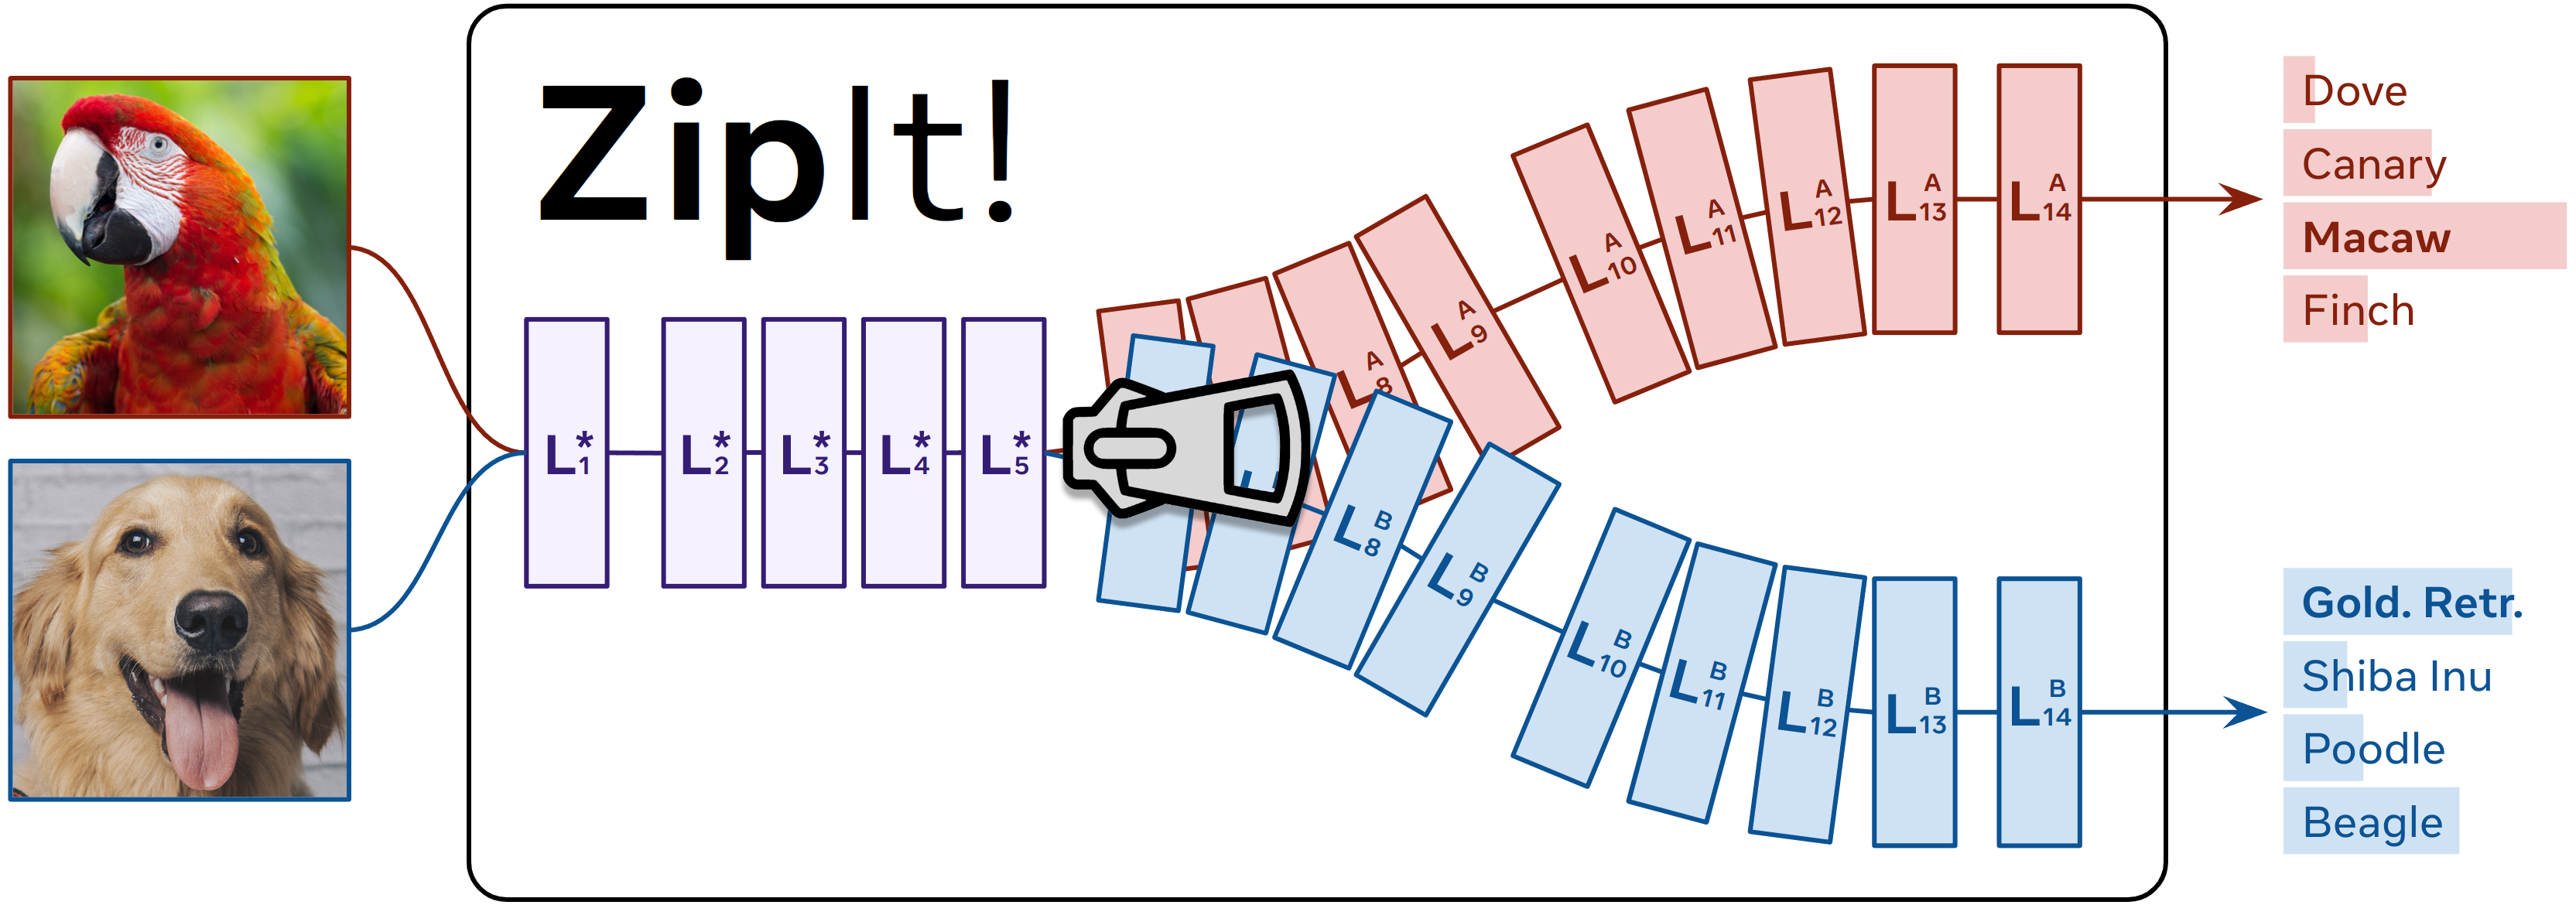
\includegraphics[width=\linewidth]{figures/imgs/concept.png}
%     \caption{{\bf \name{}} merges models trained on completely separate tasks \textit{without any additional training} by identifying their shared features.
%     Depending on the architecture and task, \name{} can nearly match their ensemble performance.
%     }
%     \label{fig:concept}
% }\end{minipage}
% \hspace{1em}
% \begin{minipage}{0.48\linewidth}{
%     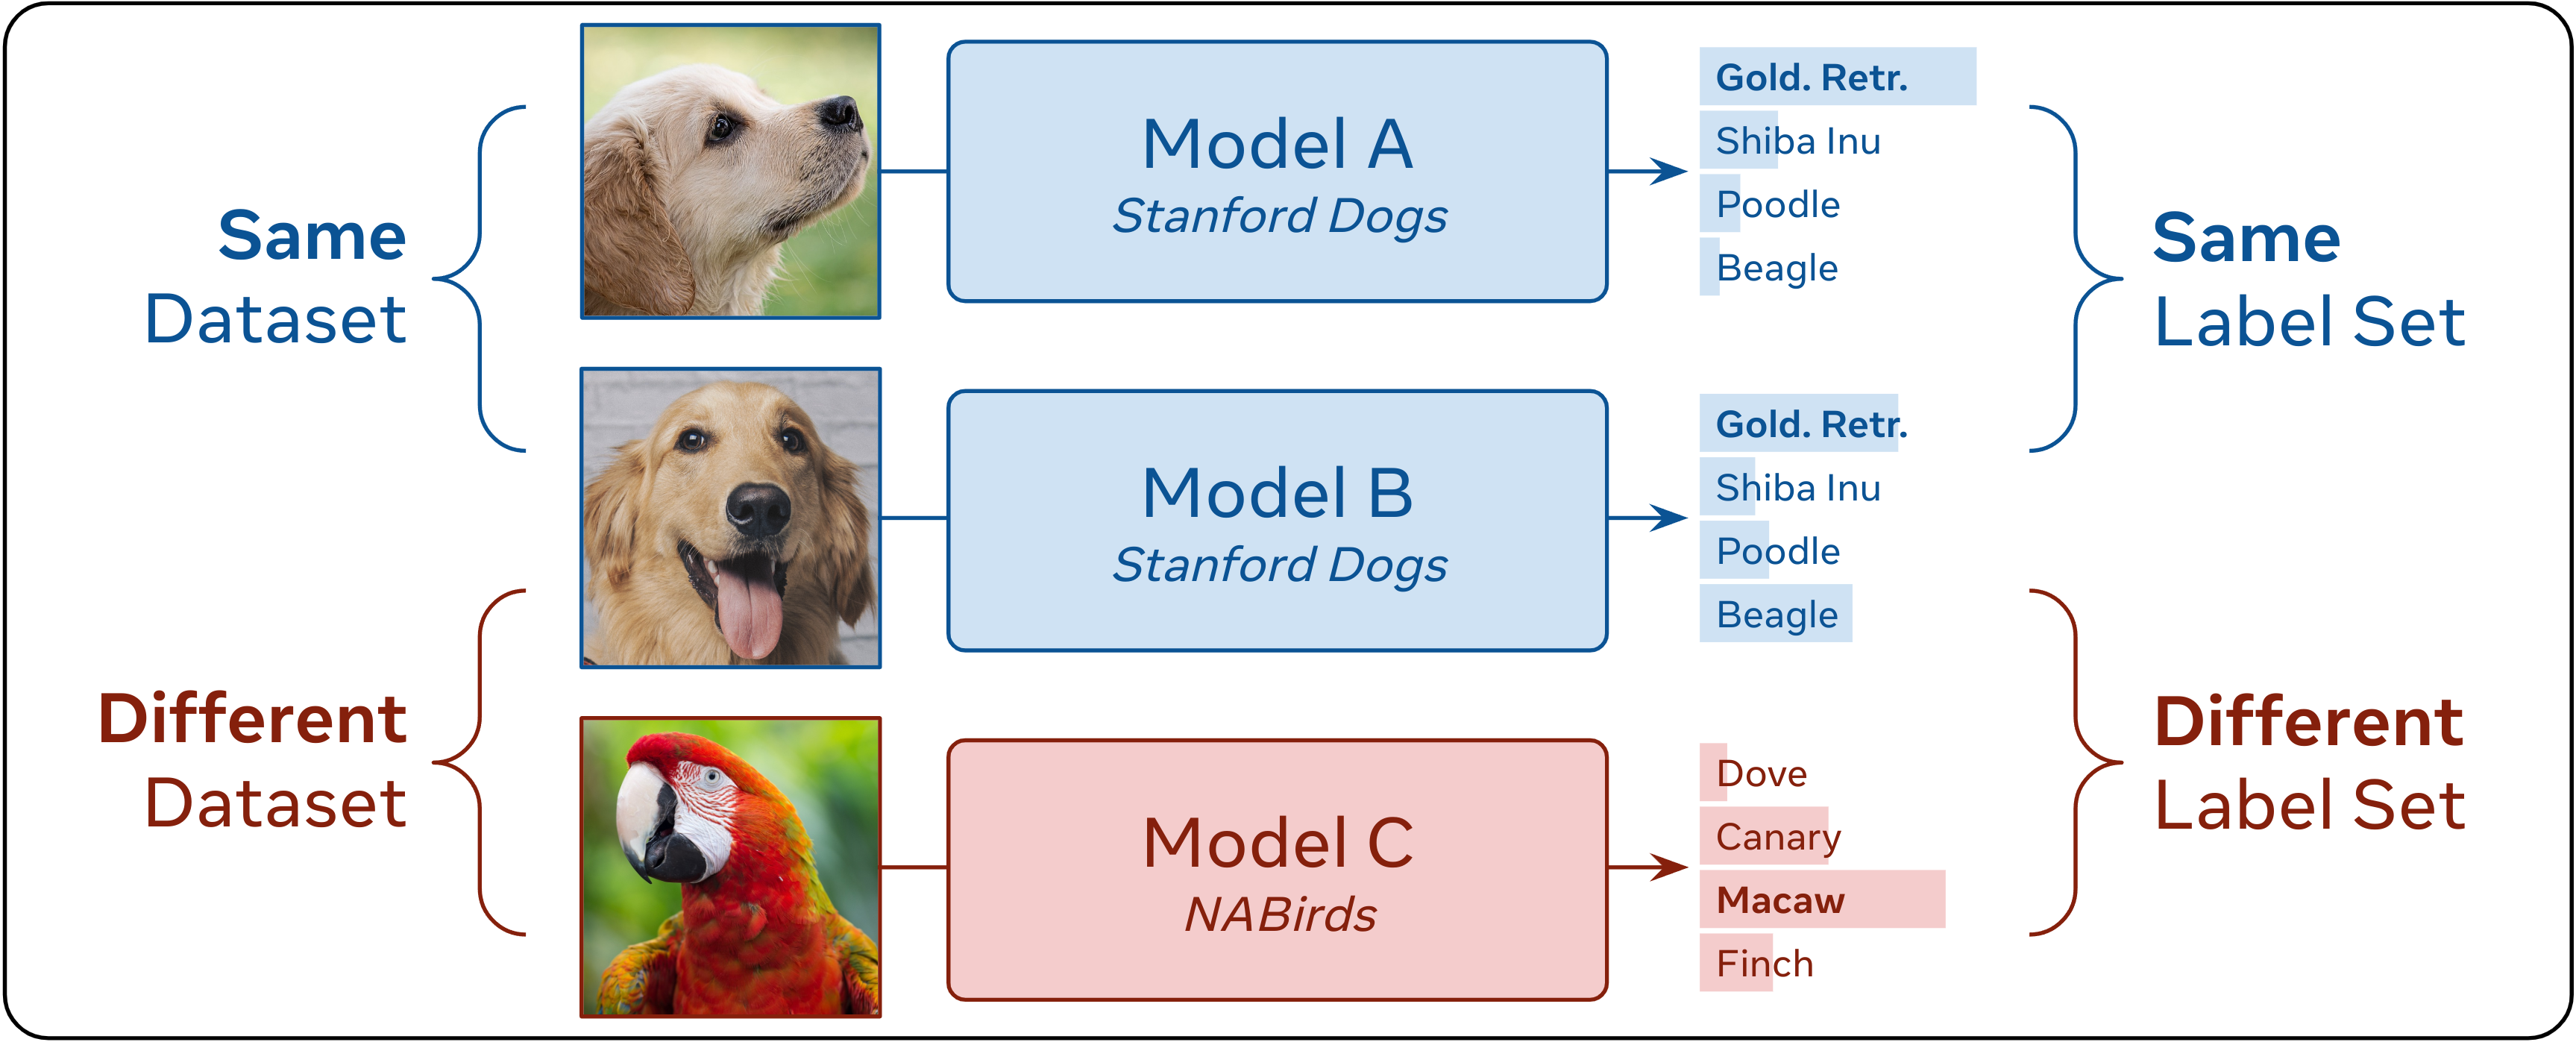
\includegraphics[width=\linewidth]{figures/imgs/vs_prior_work.png}
%     \caption{{\bf Our Setting.} Prior work \cite{wortsman2022model,ainsworth2022git,jordan2022repair}
%     focuses on merging models from the \modelb{\textbf{same} dataset} with the \modelb{\textbf{same} label sets}: e.g., merging two models both trained to classify dog breeds. In this work, we remove that restriction and ``zip'' models that can come from \modela{\textbf{different} datasets} and have \modela{\textbf{different} label sets}: e.g., merging a model that classifies dog breeds with one that classifies bird species.
%     }
%     \label{fig:capabilities}
%     % \includegraphics[width=\linewidth]{figures/imgs/random_r_experiment.png}
    
%     % \captionof{figure}{\textbf{Token Merging Schedule.} Our default constant merging schedule is close to optimal when compared to 15k randomly sampled merging schedules on an AugReg ViT-B/16. }
%     % \label{fig:r_ablation}
% }\end{minipage}
% \end{figure}


% #########################################################
